%--------------------------------------------------------------------------
%	PACKAGES AND THEMES
%--------------------------------------------------------------------------
\documentclass{beamer}
\usepackage[utf8]{inputenc}

\usetheme{Madrid}
\usecolortheme{default}
\setbeamertemplate{navigation symbols}{}

\usepackage{hyperref}
\usepackage{graphicx} % Allows including images
\usepackage{booktabs} % Allows the use of \toprule, \midrule and \bottomrule in tables

%--------------------------------------------------------------------------
%	TITLE PAGE
%--------------------------------------------------------------------------

% The title
\title{Vizualizacija Kakeya-množice}
\subtitle{Generiranje slik s programskim orodjem Ipe}

\author{Terezija Krečič}
\institute[FMF] % Your institution may be shorthand to save space
{
    % Your institution for the title page
    Fakulteta za matematiko in fiziko \\
    Pedagoška matematika 
    \vskip 3pt
}
\date{29. maj 2024} % Date, can be changed to a custom date


%--------------------------------------------------------------------------
%	PRESENTATION SLIDES
%--------------------------------------------------------------------------

\begin{document}

\begin{frame}
    % Print the title page as the first slide
    \titlepage
\end{frame}

%------------------------------------------------

\begin{frame}{Problem, ki ga rešujemo}
    \begin{alertblock}{Vprašanje Kakeye (1917)}
        Kolikšna je lahko najmanjša ploščina območja, znotraj katerega se daljica dolžine 1 zvezno obrne za 360°?
    \end{alertblock}
    \pause
    Matematiki, ki so prispevali k rešitvi:
    \begin{itemize}
        \item Abram Besicovitch (RUS)
        \item Oskar Perron (NEM)
        \item Gyula Pál (MADŽ-DAN)
    \end{itemize}
\end{frame}

%------------------------------------------------

\begin{frame}{Konstrukcija -- s čim začnemo}
    \begin{figure}
        \centering
        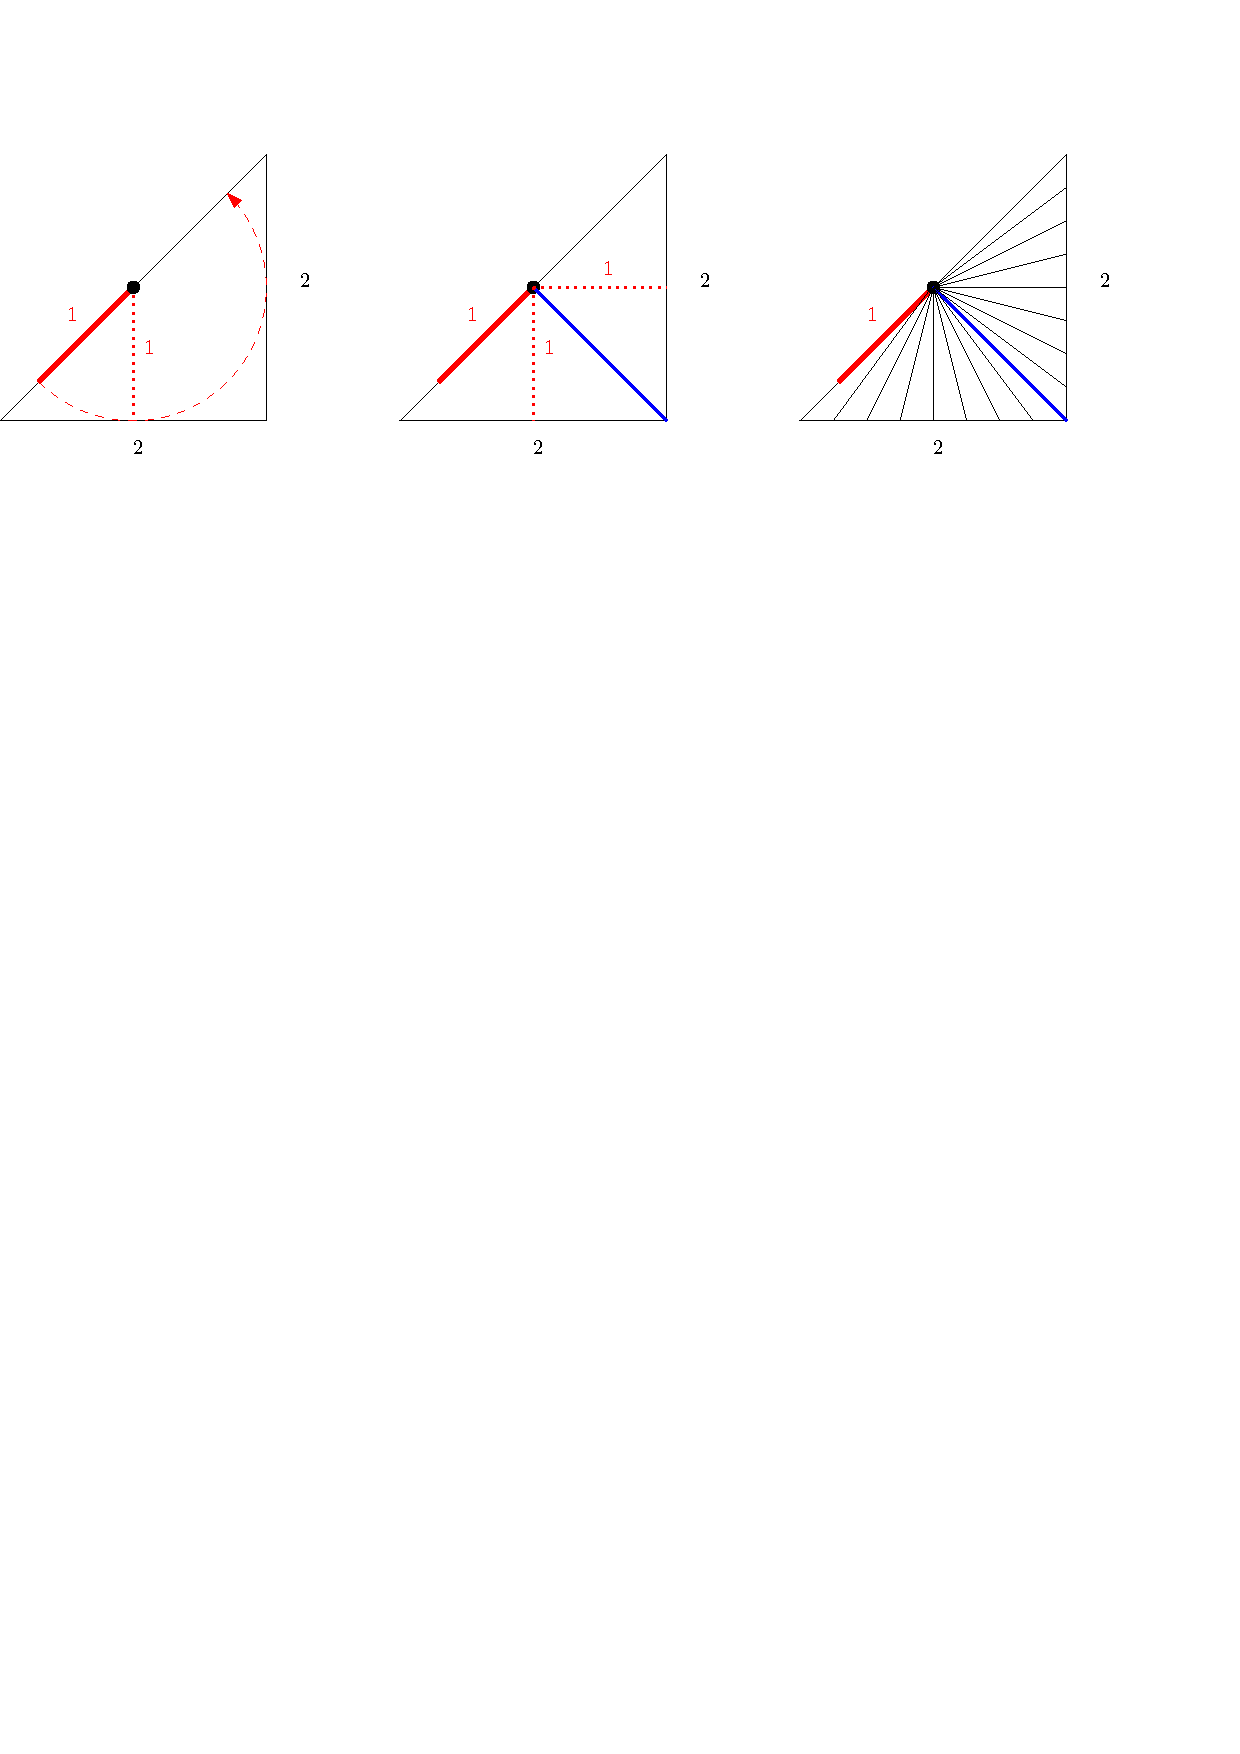
\includegraphics[width=0.9\textwidth]{ipe_slike/trikotnik_razdelitev.pdf}
    \end{figure}
\end{frame}

%------------------------------------------------

\begin{frame}{Konstrukcija -- translacije podtrikotnikov}
    \begin{figure}
        \centering
        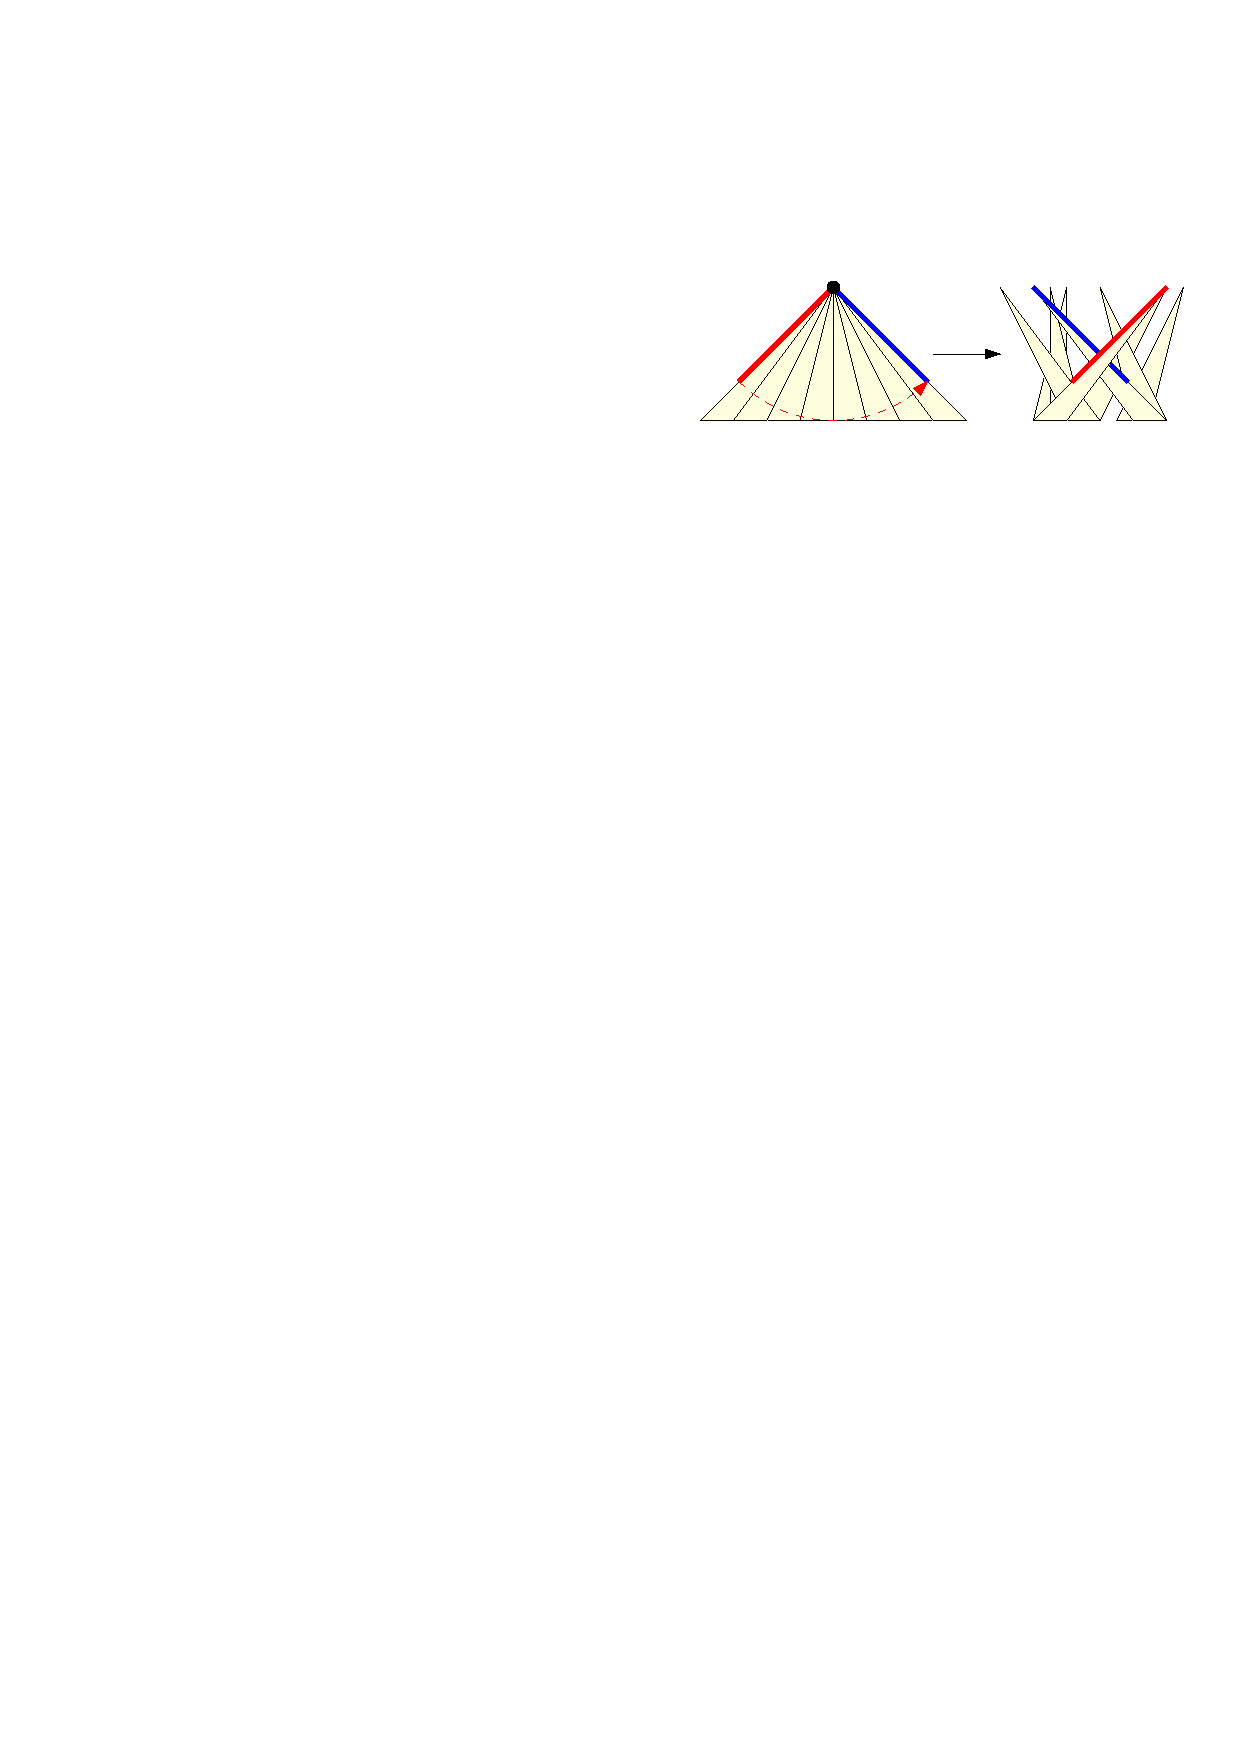
\includegraphics[width=0.7\textwidth]{ipe_slike/translacija_podtrikotnikov.pdf}
        \pause
        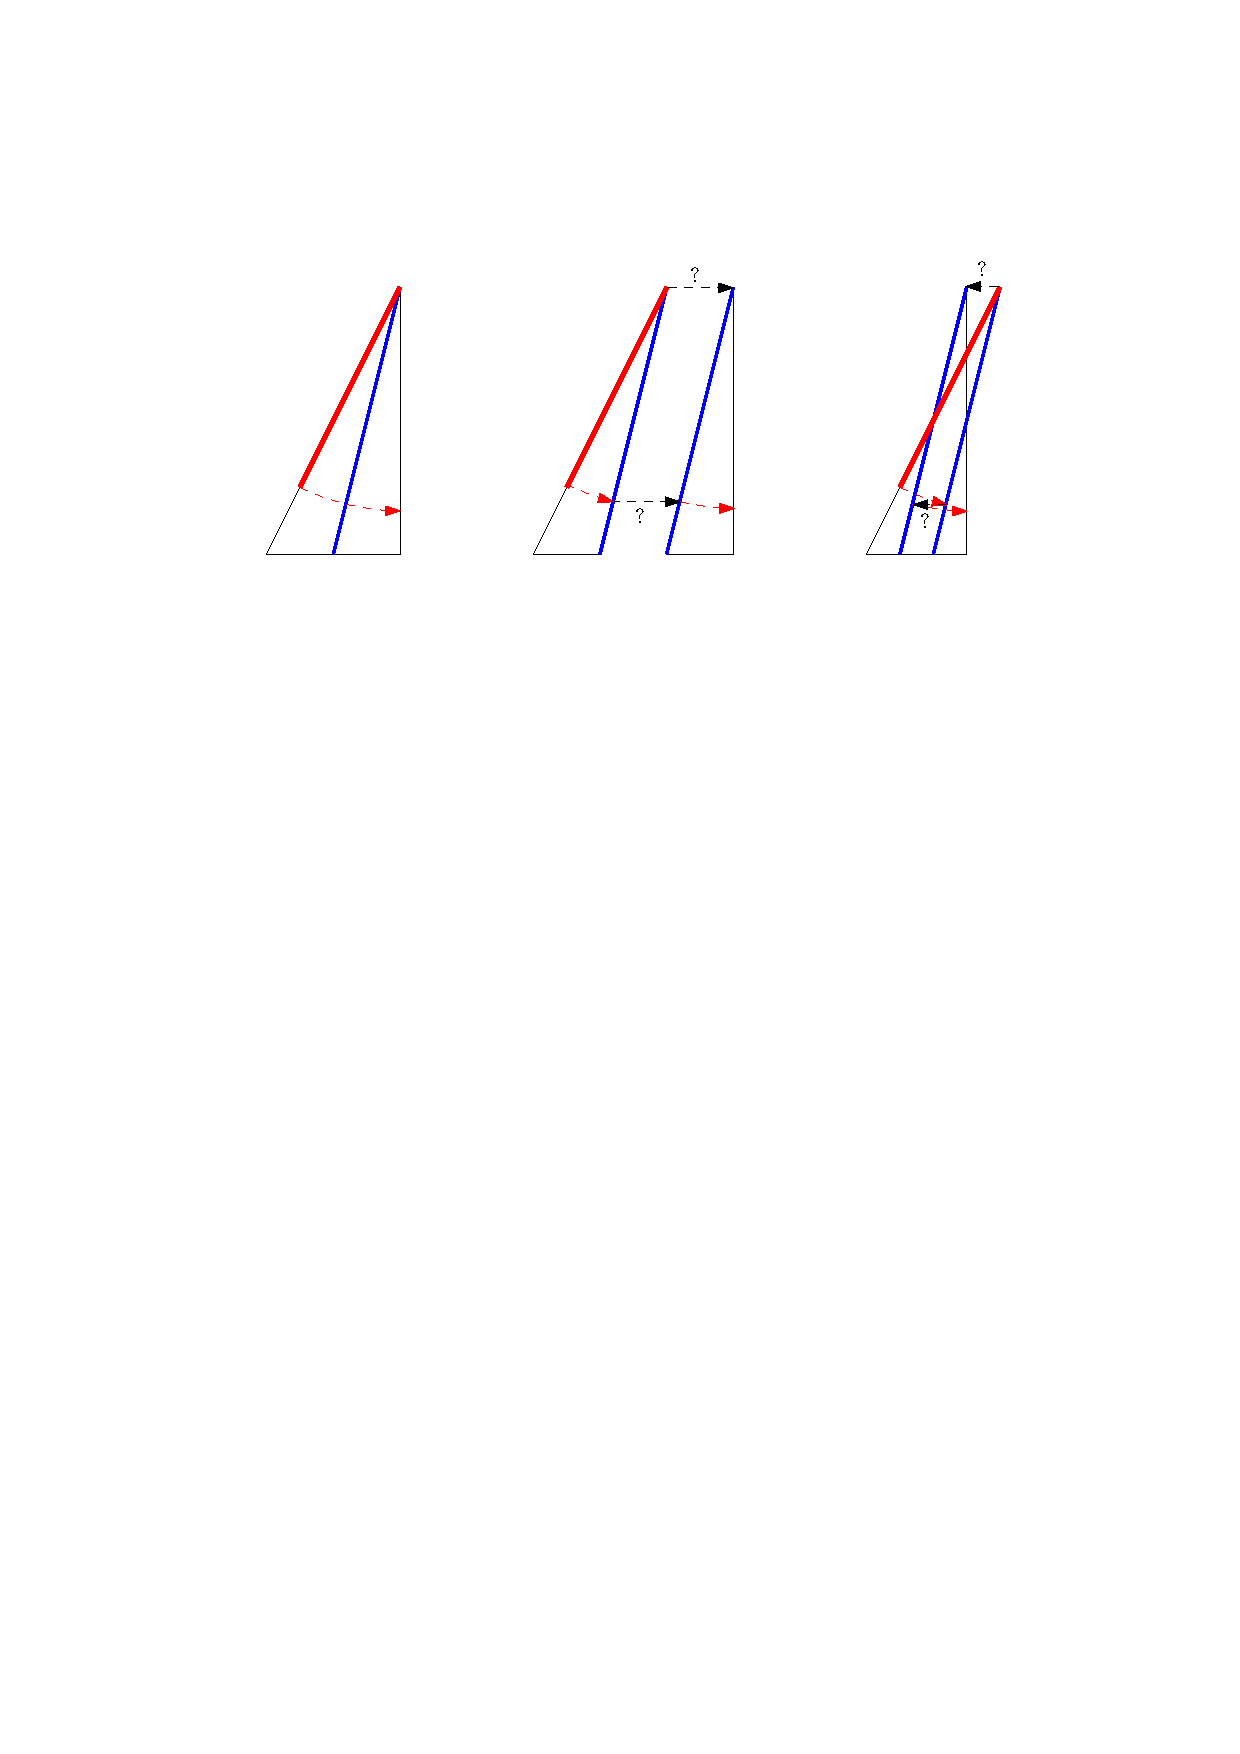
\includegraphics[width=0.7\textwidth]{ipe_slike/preskok1.pdf}
    \end{figure}
\end{frame}

%------------------------------------------------

\begin{frame}{Konstrukcija -- Pálov spoj}
    \begin{figure}
        \centering
        \includegraphics<1>[width=0.5\textwidth]{ipe_slike/pal1.pdf}
        \includegraphics<2>[width=0.5\textwidth]{ipe_slike/pal2.pdf}
    \end{figure}
\end{frame}

%------------------------------------------------

\begin{frame}{Perronovo drevo}
    \begin{figure}
        \centering
        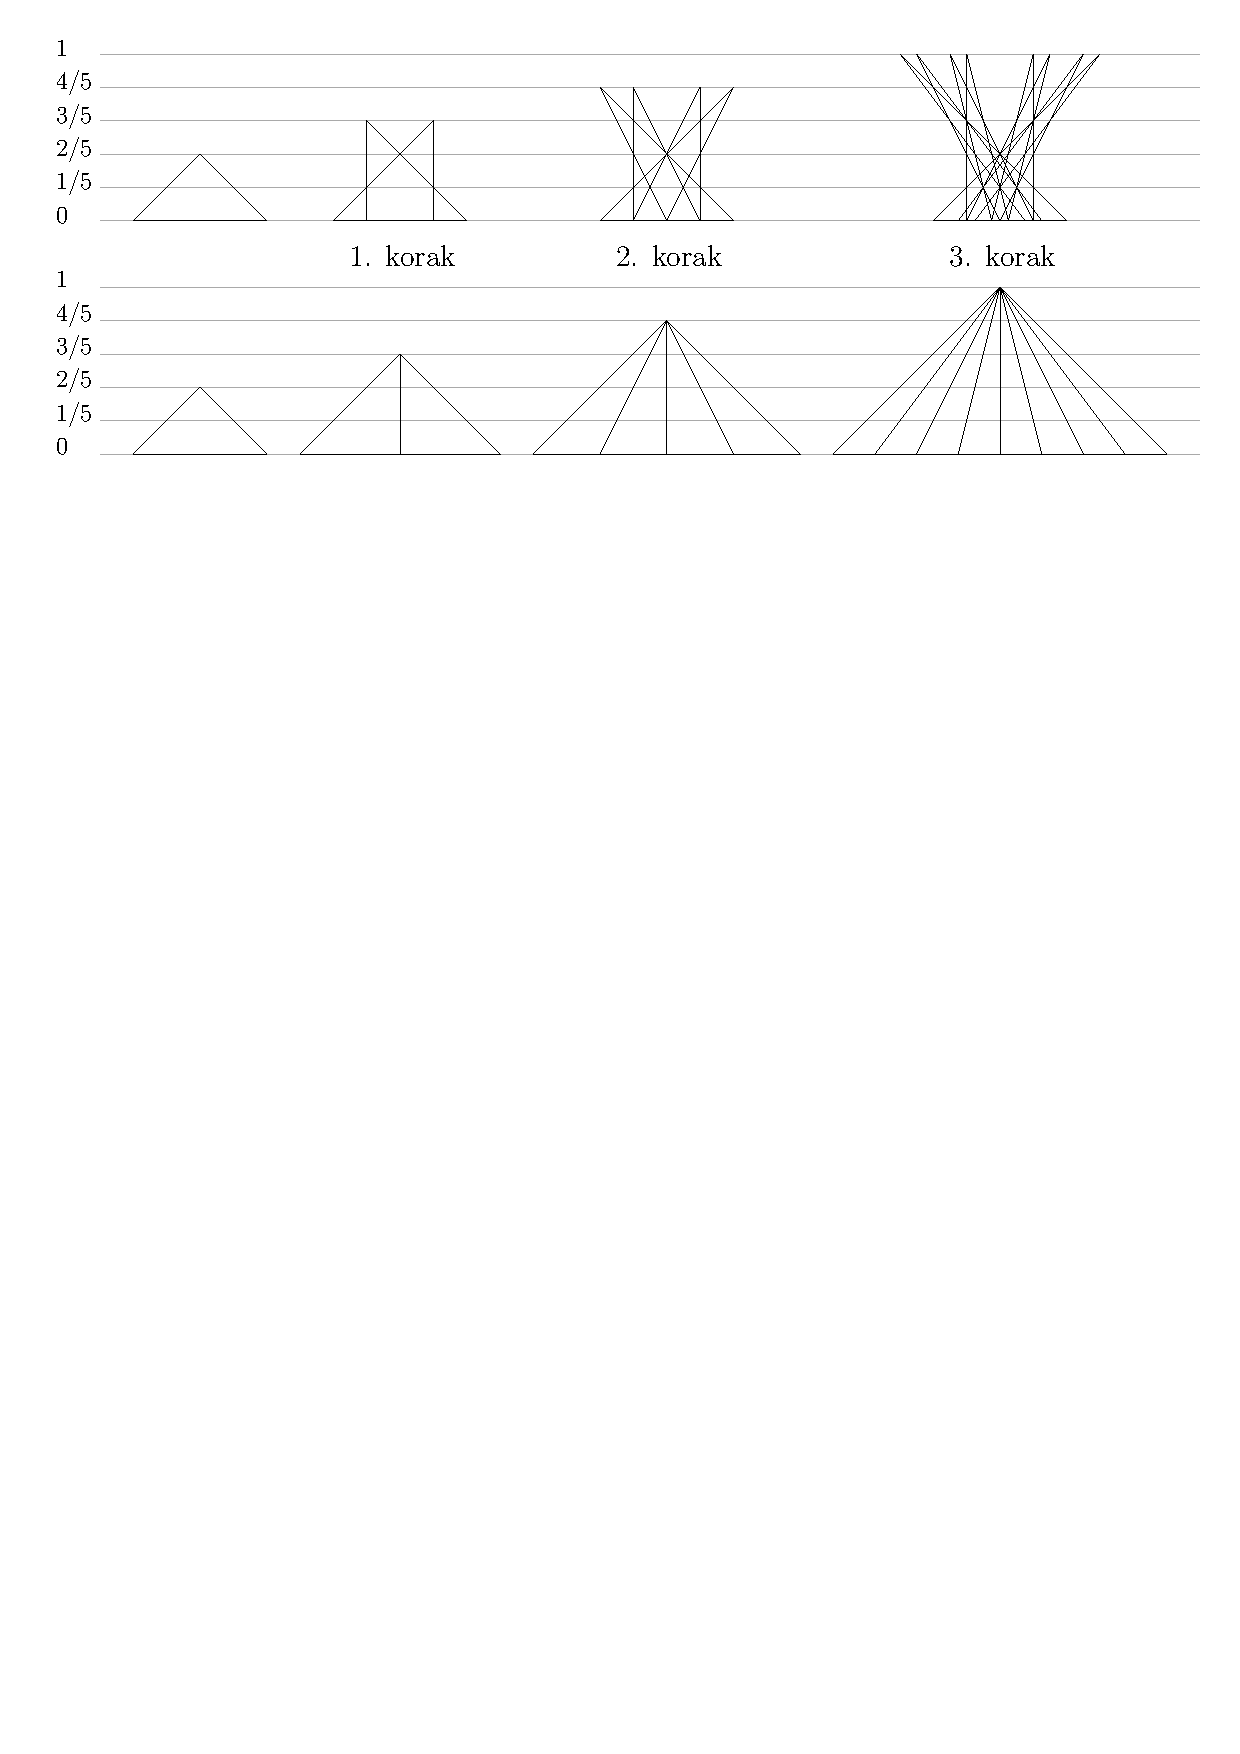
\includegraphics[width=0.9\textwidth]{ipe_slike/lastnost2.pdf}
    \end{figure}
\end{frame}

%------------------------------------------------

\begin{frame}{Lastnosti pri brstenju Perronovega drevesa}
    \begin{enumerate}
        \item Vsak vrh porodi skadna uhlja, ki imata enako ploščino kot taisti vrh.
        \pause \item V $ l $-tem koraku ($ l = 1, 2, \ldots, k-2 $) dobimo $ 2^l $ prekrivajočih se podtrikotnikov, ki skupaj sestavijo osnovnemu trikotniku podoben trikotnik z višino $ \frac{l+2}{k} $.
        \pause \item V vsakem koraku se nam skupna ploščina poveča za natanko dvakratno ploščino vrha, s katerim začnemo prvi korak, tj. za $ \frac{2}{k^2} $.
        \pause \item Skupna ploščina lika, ki ga dobimo na zadnjem koraku, je $ \frac{2}{k} $.
    \end{enumerate}
\end{frame}

%------------------------------------------------

\begin{frame}{Povzetek konstrukcije}
    \begin{enumerate}
        \item pravokotni enakostranični trikotnik z višino 1
        \item $ k \in \mathbb{N} \backslash \{1\} \rightarrow n = 2^{k-2} $ podtrikotnikov
        \item Perronovo drevo s ploščino $ \frac{2}{k} $
    \end{enumerate}
    \begin{figure}
        \centering
        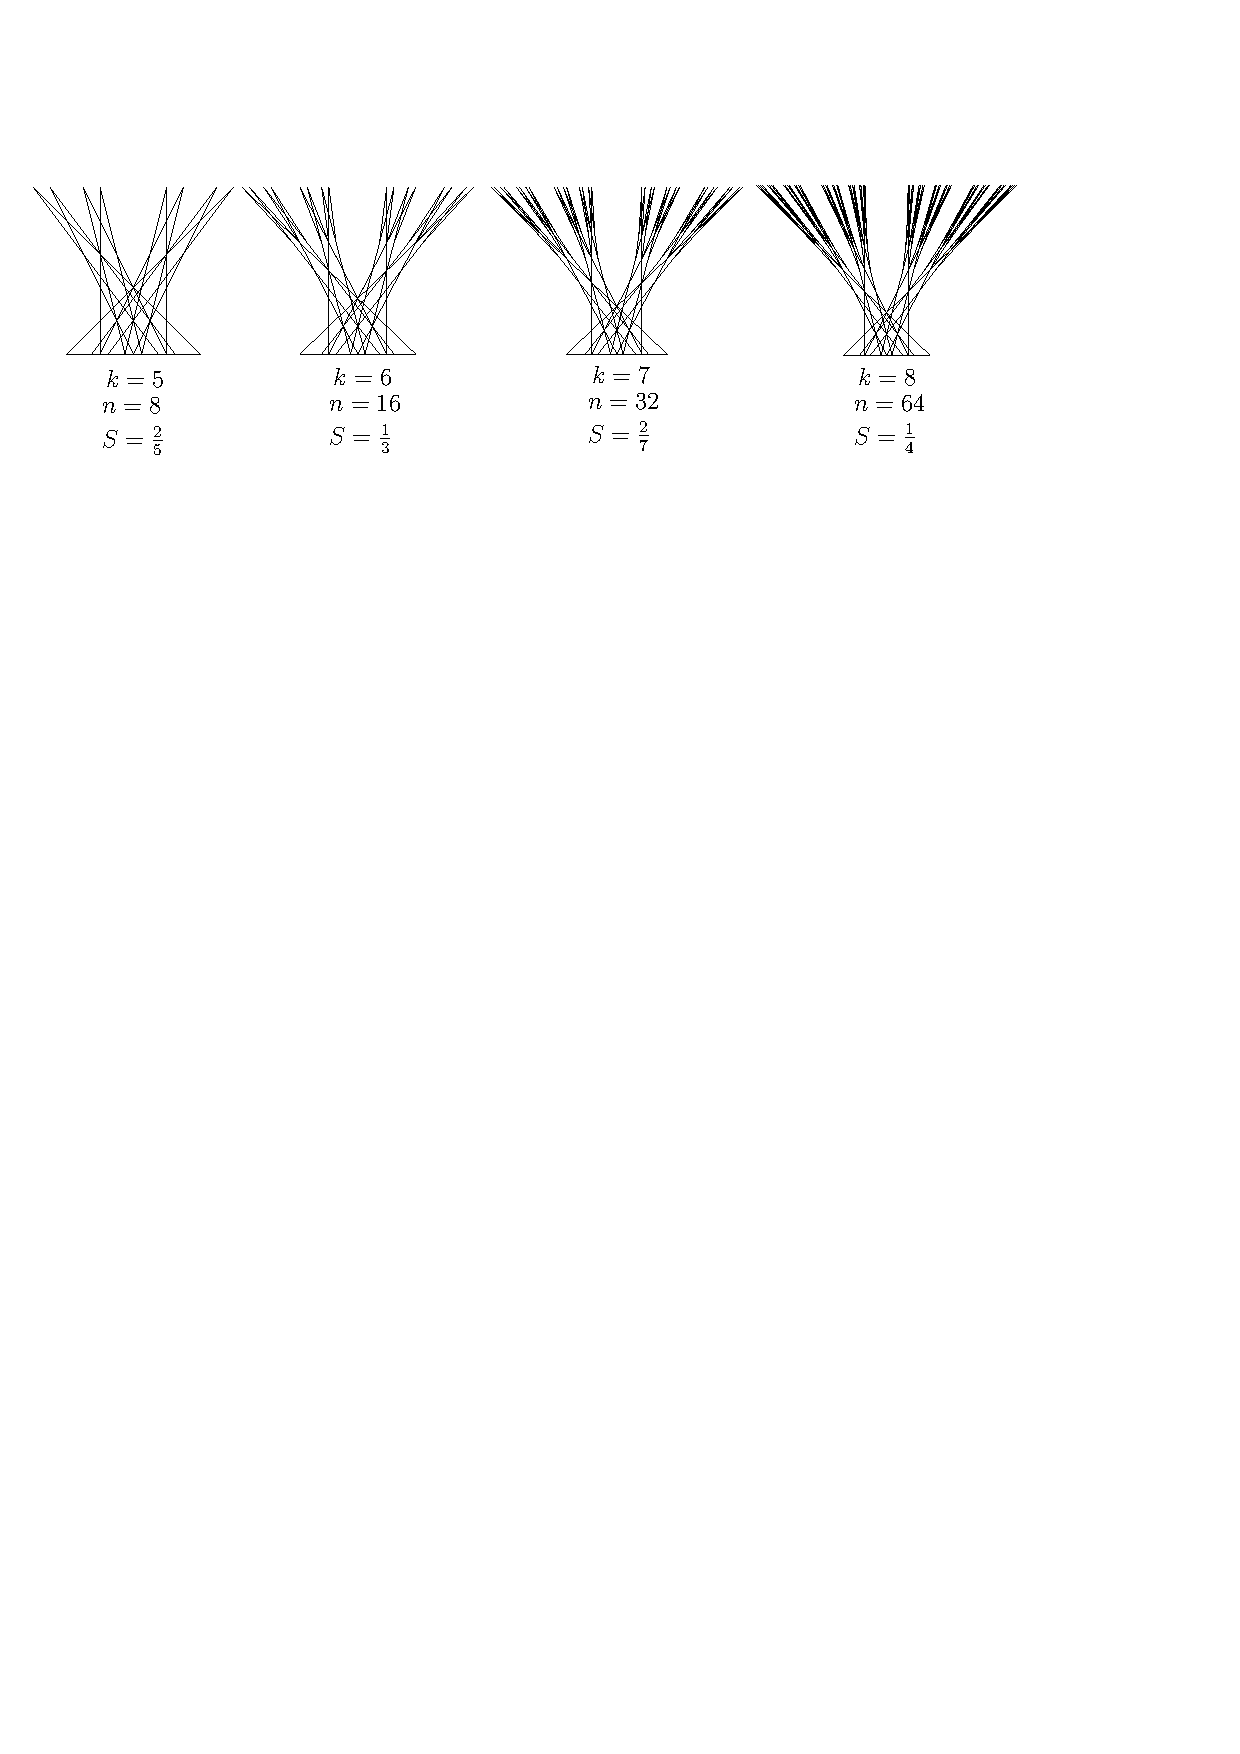
\includegraphics[width=\textwidth]{ipe_slike/brstenje_k_n.pdf}
    \end{figure}
\end{frame}

%------------------------------------------------

\begin{frame}{Povzetek konstrukcije}
    \begin{figure}
        \centering
        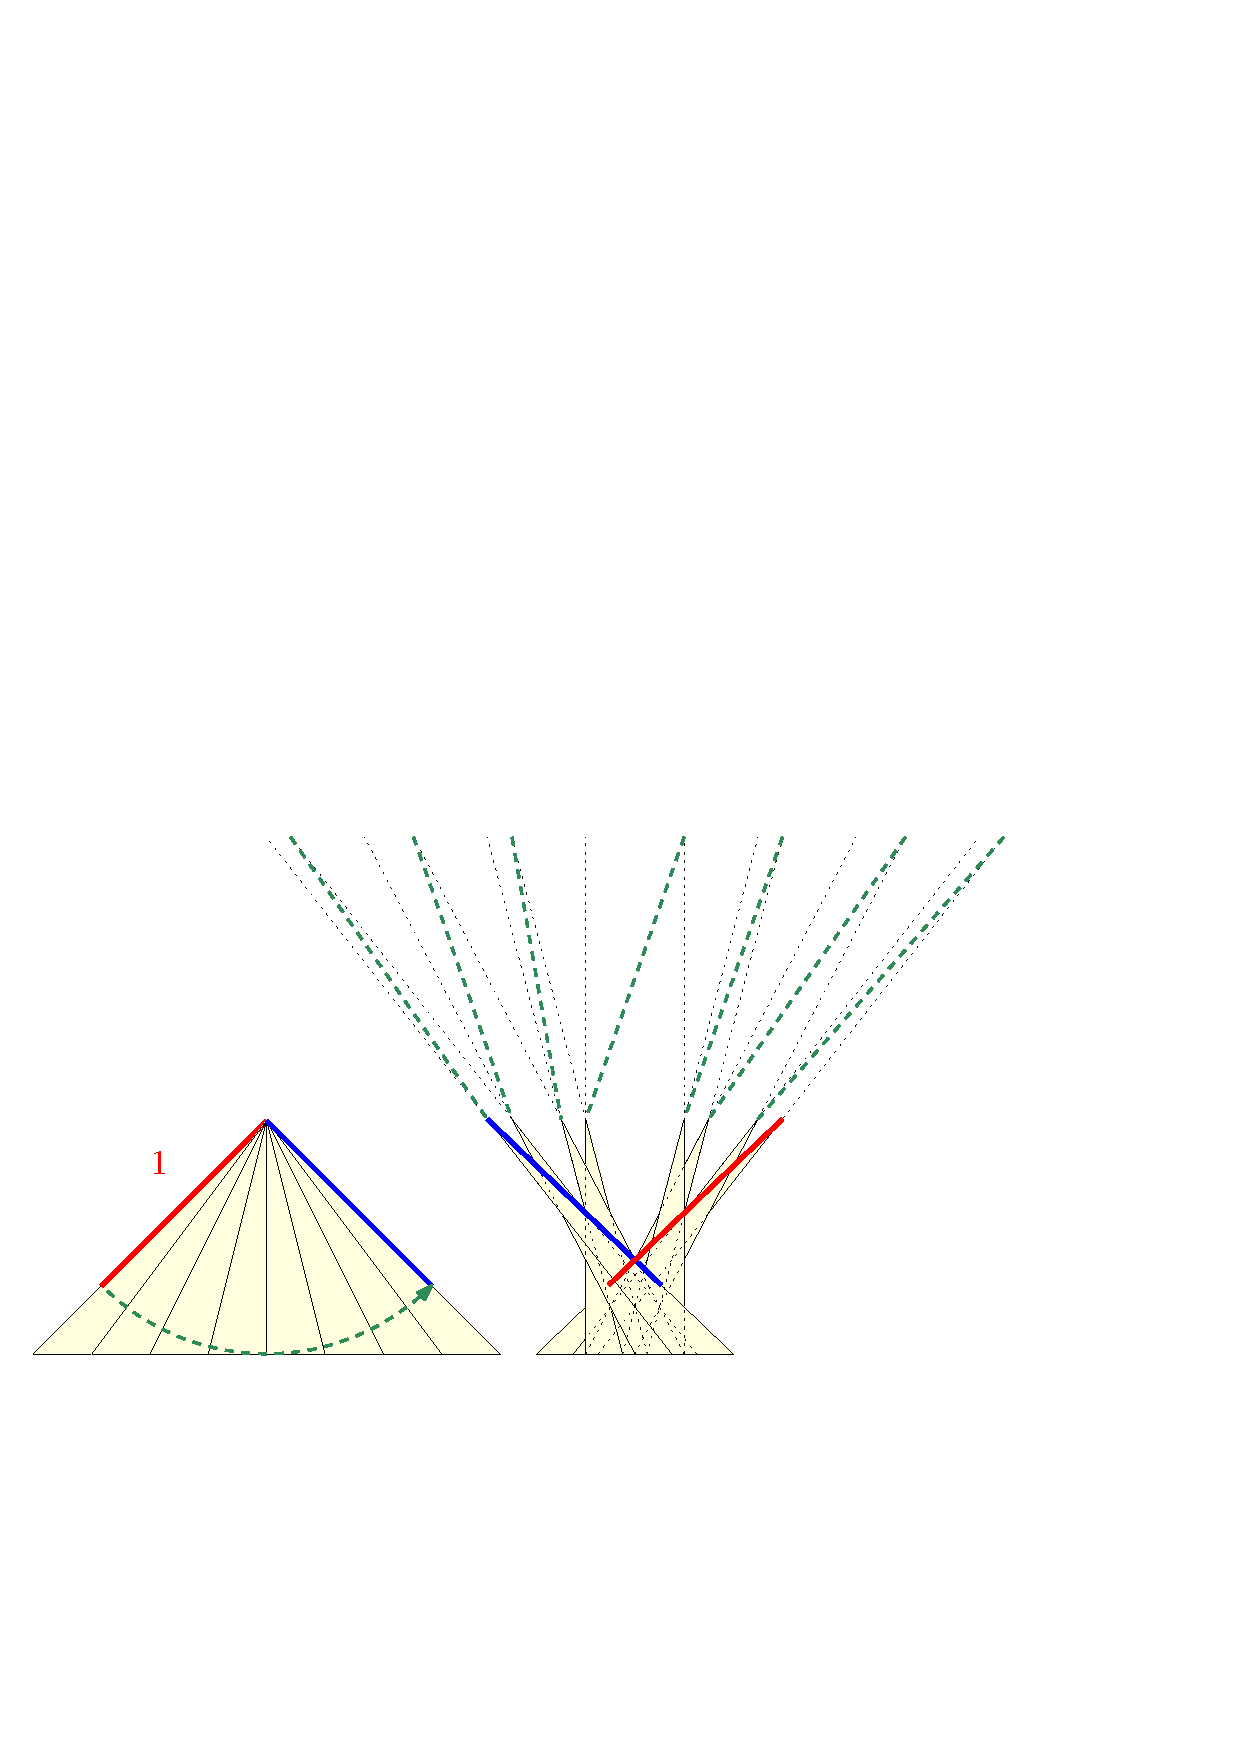
\includegraphics[width=\textwidth]{ipe_slike/prehod_drevo1.pdf}
    \end{figure}
    \pause
    Ploščina: $ \frac{2}{k} + (n-1) \epsilon = \frac{2}{k} + (2^{k-2} - 1) \epsilon $
\end{frame}

%------------------------------------------------

\begin{frame}{Združimo v Kakeya-množico}
    \begin{figure}
        \centering
        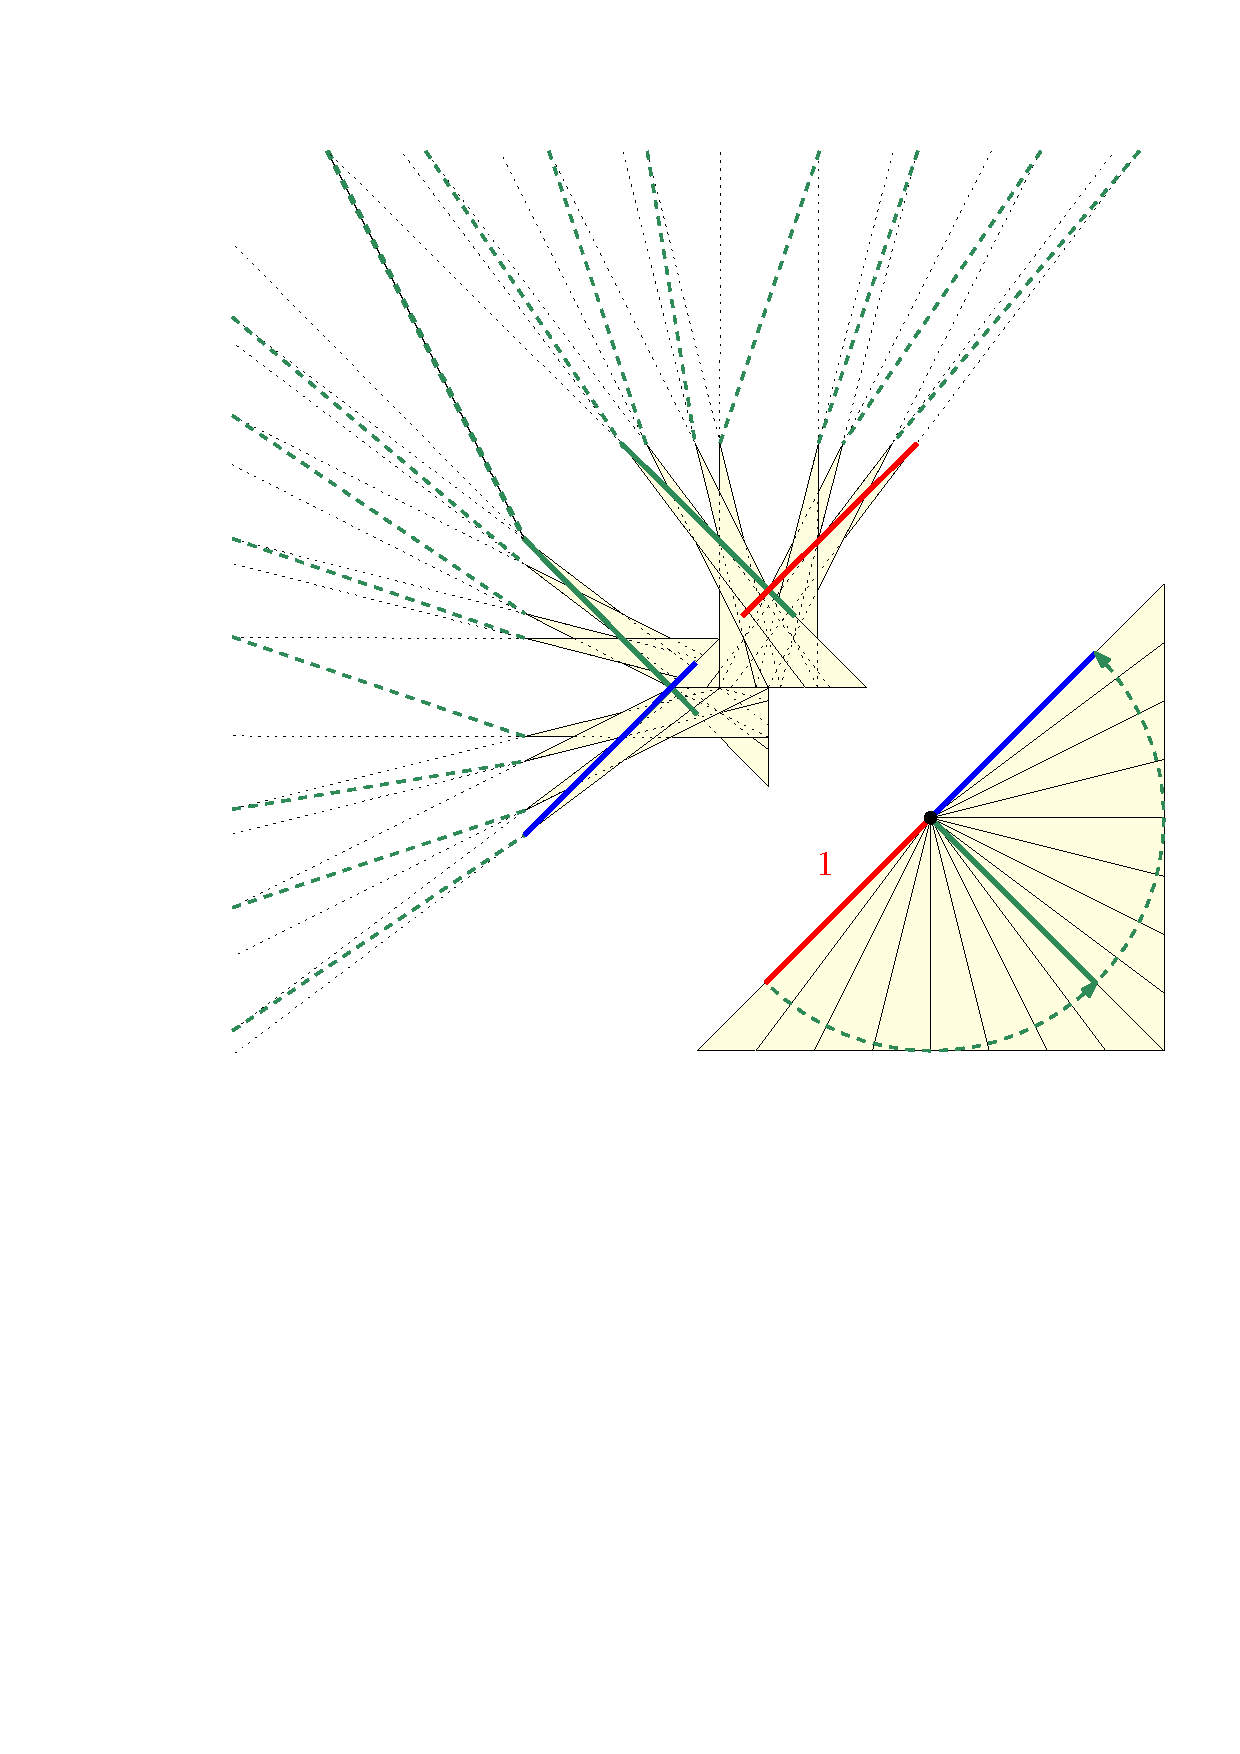
\includegraphics[width=0.6\textwidth]{ipe_slike/prehod_skupaj.pdf}
    \end{figure}
\end{frame}

\begin{frame}{Združimo v Kakeya-množico}
    \begin{figure}
        \centering
        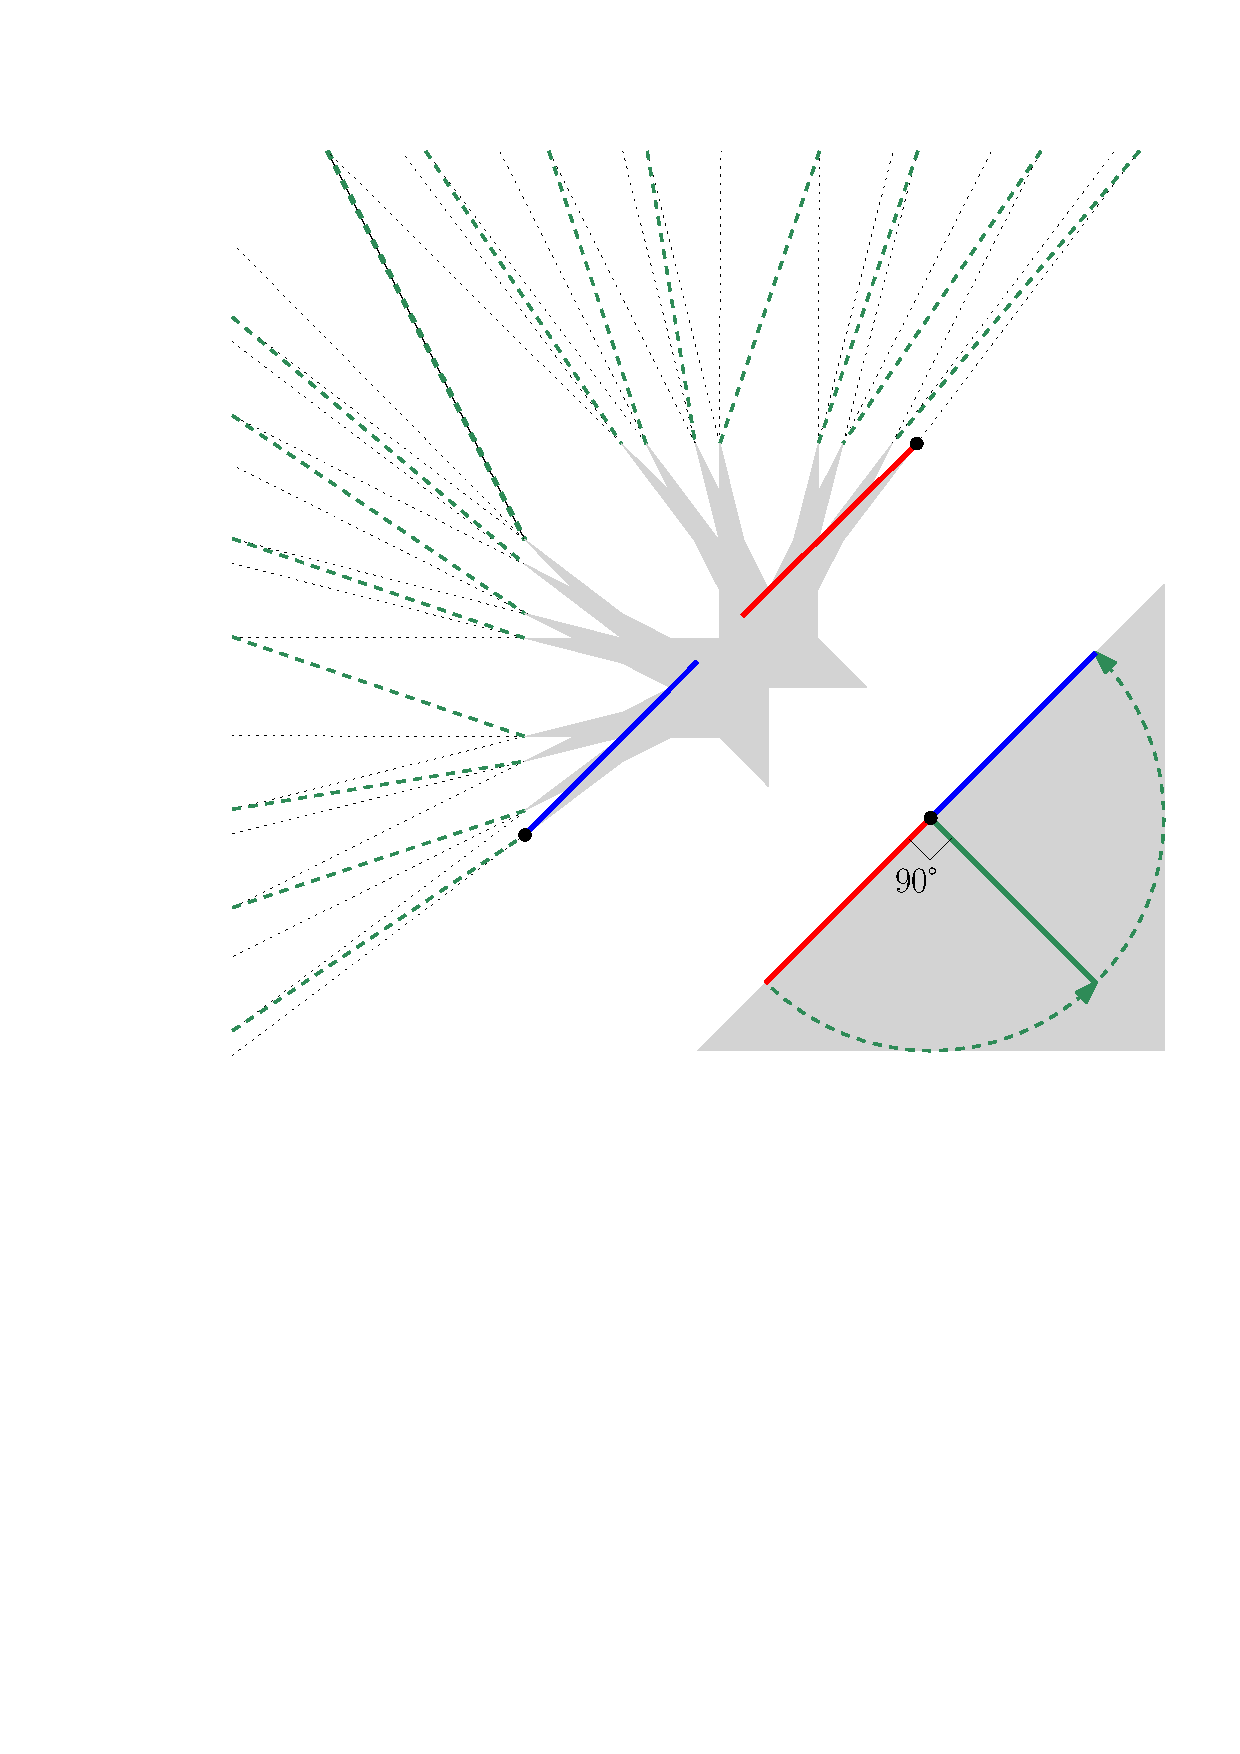
\includegraphics[width=0.6\textwidth]{ipe_slike/koncni_lik_90.pdf}
    \end{figure}
    $ S_{90} = 2 \cdot \left( \frac{2}{k} + (2^{k-2} - 1) \epsilon \right) + \epsilon = \frac{4}{k} + (2^{k-1} - 1) \epsilon  \rightarrow $ \textcolor{red}{\textbf{poljubno majhna!}}
\end{frame}

%------------------------------------------------

\begin{frame}{Ena od alternativnih rešitev}
    \begin{figure}
        \centering
        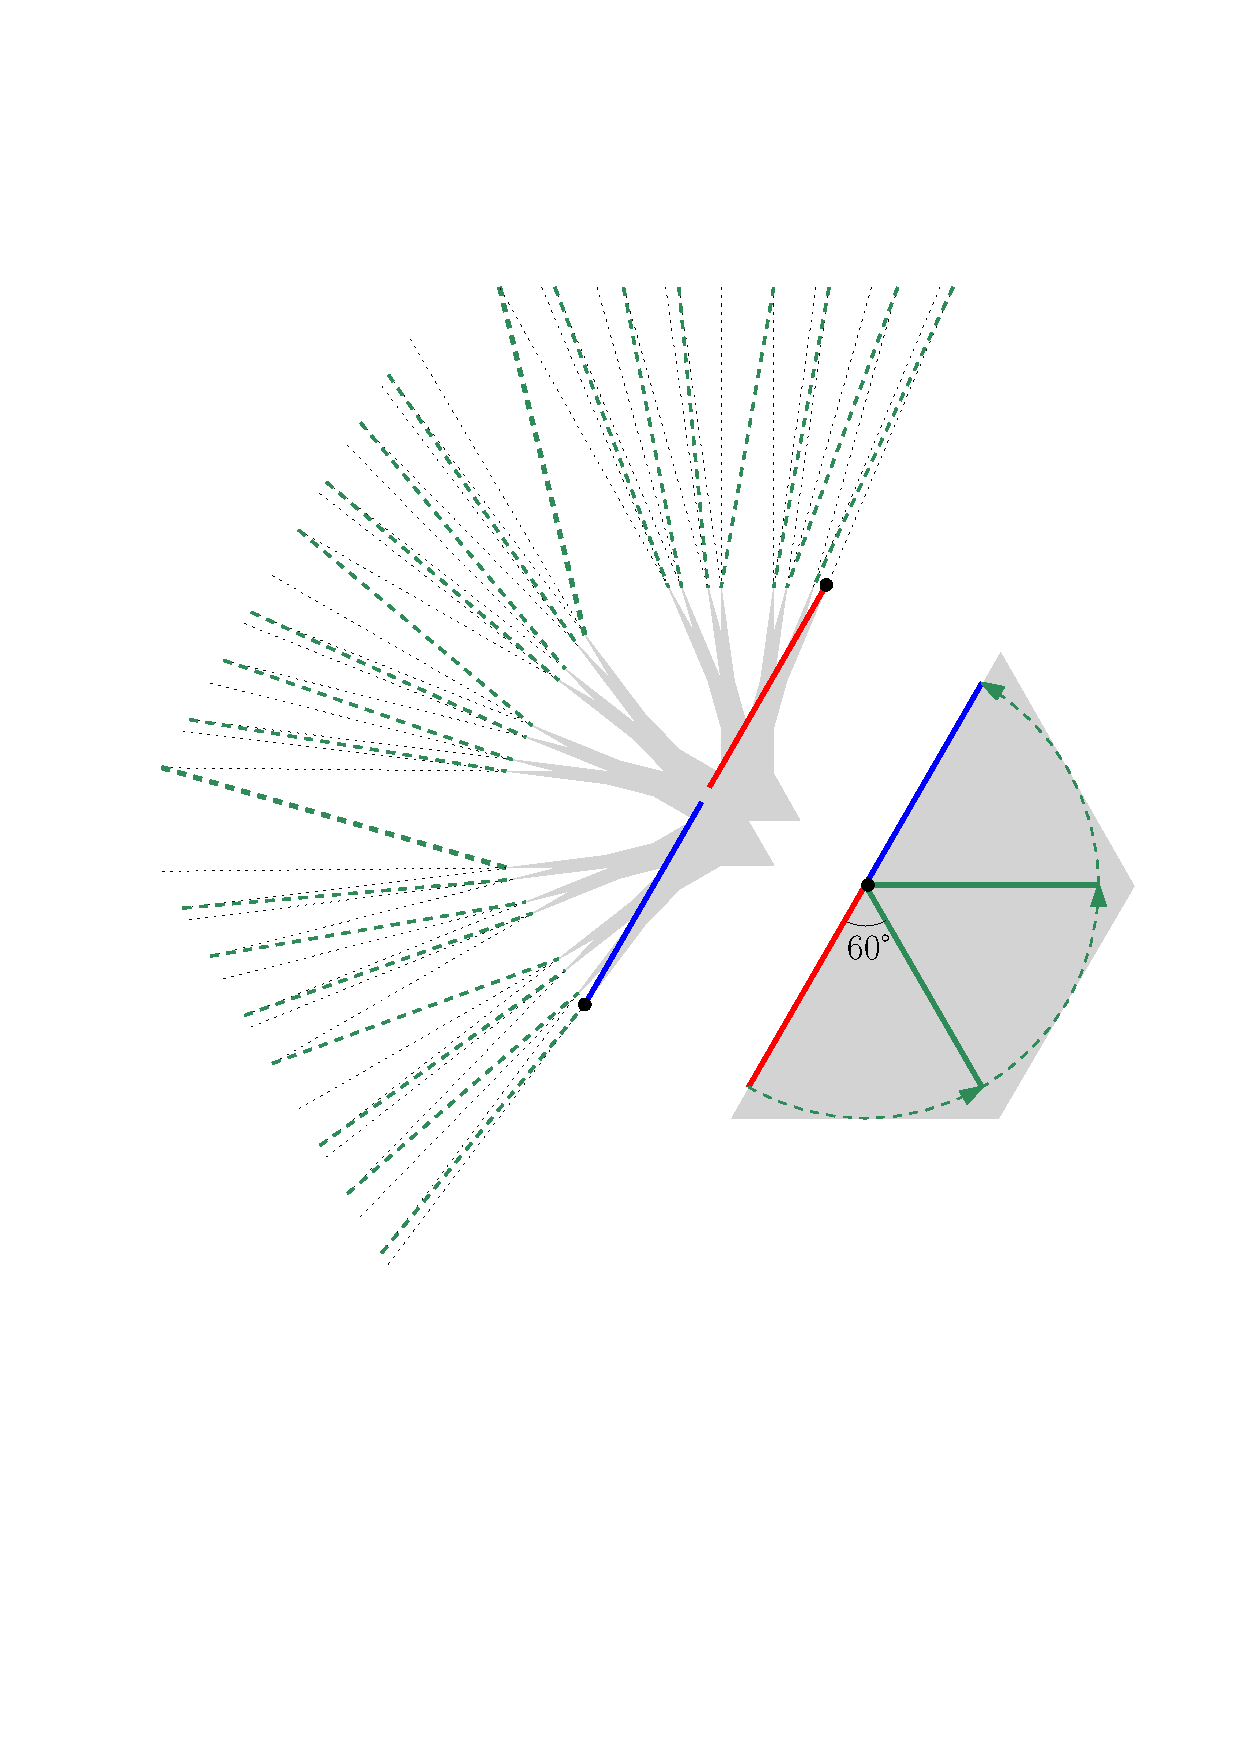
\includegraphics[width=0.55\textwidth]{ipe_slike/koncni_lik_60.pdf}
    \end{figure}
    $ S_{60} = 3 \cdot \left( \frac{k+2}{k^2 \sqrt{3}} + (2^{k-2} - 1) \epsilon \right) + 2\epsilon = \frac{\sqrt{3} (k+2)}{k^2} + (3 \cdot 2^{k-2} -1) \epsilon $

\end{frame}

%------------------------------------------------

\begin{frame}{Vir}
    \nocite{*}      % navede tudi vire, ki jih ne citiras
    \bibliographystyle{ieeetr}
    \bibliography{literatura.bib}
\end{frame}

%------------------------------------------------

\end{document}